\documentclass[12pt]{article}
%\documentclass{article}

\usepackage{times}
\usepackage[final]{graphicx}
\usepackage{hyperref}

\setlength{\topmargin}{-0.5in}
\setlength{\oddsidemargin}{0in}
\setlength{\evensidemargin}{0in}
\setlength{\textwidth}{6.5in}
\setlength{\textheight}{9.0in}

\begin{document}

\centerline{\bf \Large CS295/CS395/CSYS395: \href{CS295_395_Syllabus.pdf}{\underline{Evolutionary Robotics}}}

\vspace{0.5cm}

\centerline{\bf \large Programming Assignment 8 of 10}

\vspace{0.5cm}

\centerline{\large Assigned: Friday, October 21, 2011}

\vspace{0.5cm}

\centerline{\large Due: Friday, October 28, 2011 by midnight}

\vspace{0.5cm}

\noindent \textbf{Description:} In this week's assignment you will add sensors to your robot. You will add one binary touch sensor in each of the four lower legs: the sensor will fire when that leg is touching the ground, and will not fire when the leg is off the ground. Adding touch sensors requires four basic steps:

\begin{enumerate}

\item Set all touch sensor values to zero at the outset of each time step of the simulation.

\item Add code so that, when nearCallback is called because there is a collision between a leg and the ground plane, ODE knows which leg collided.

\item Set the touch for that leg to 1.

\item For those legs touching the ground, paint them black; those that do not touch the ground, paint white (see Fig. \ref{Fig1}).
\end{enumerate}

\begin{figure}
\centerline{
a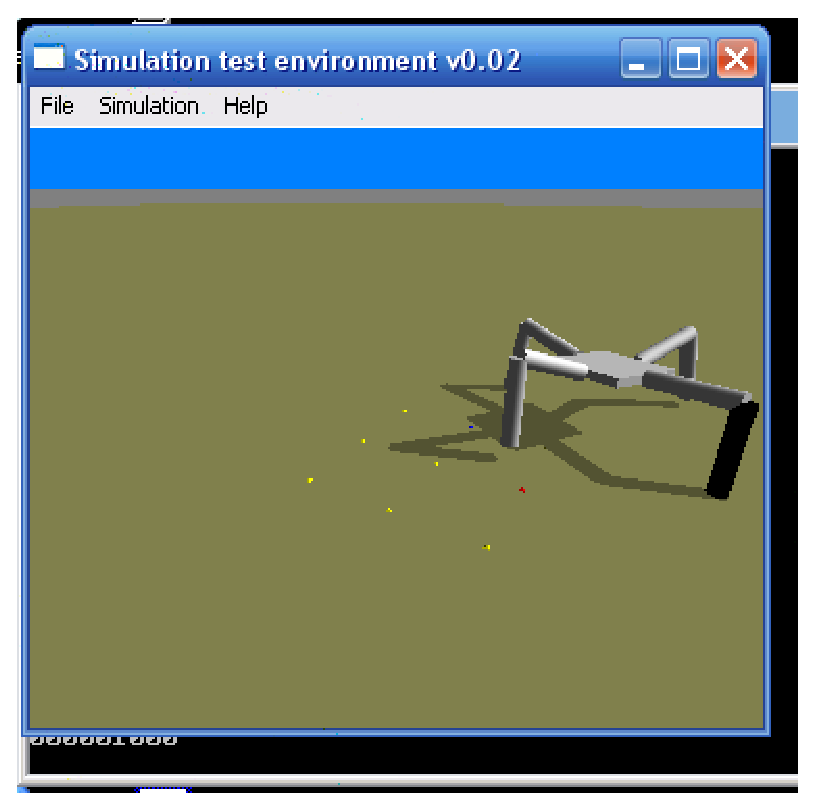
\includegraphics[height=5cm]{Quad1}
b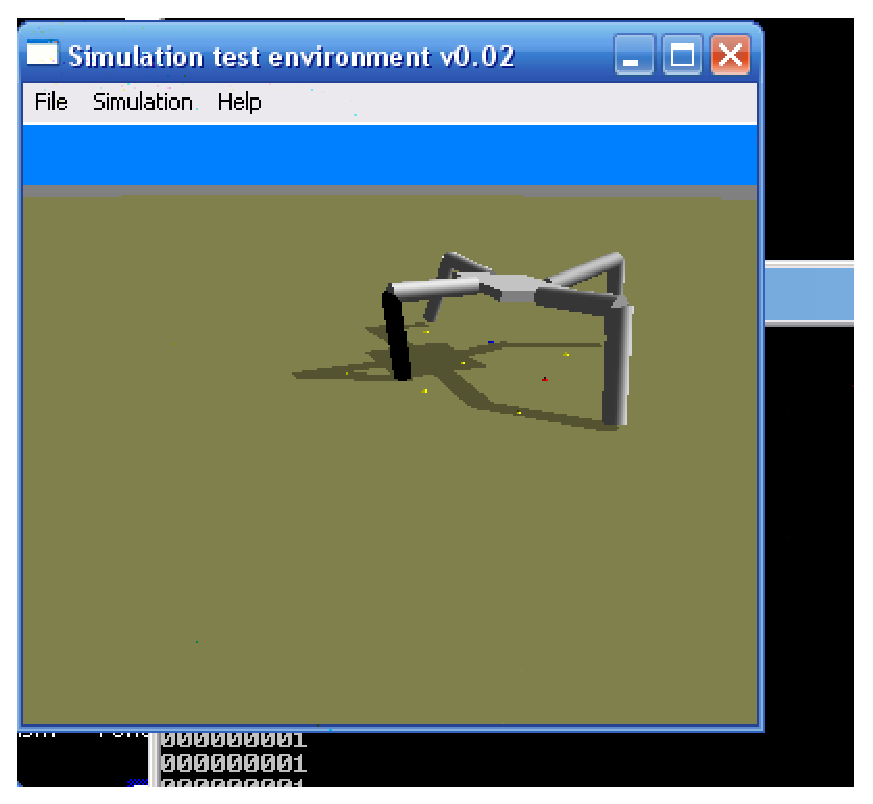
\includegraphics[height=5cm]{Quad2}
c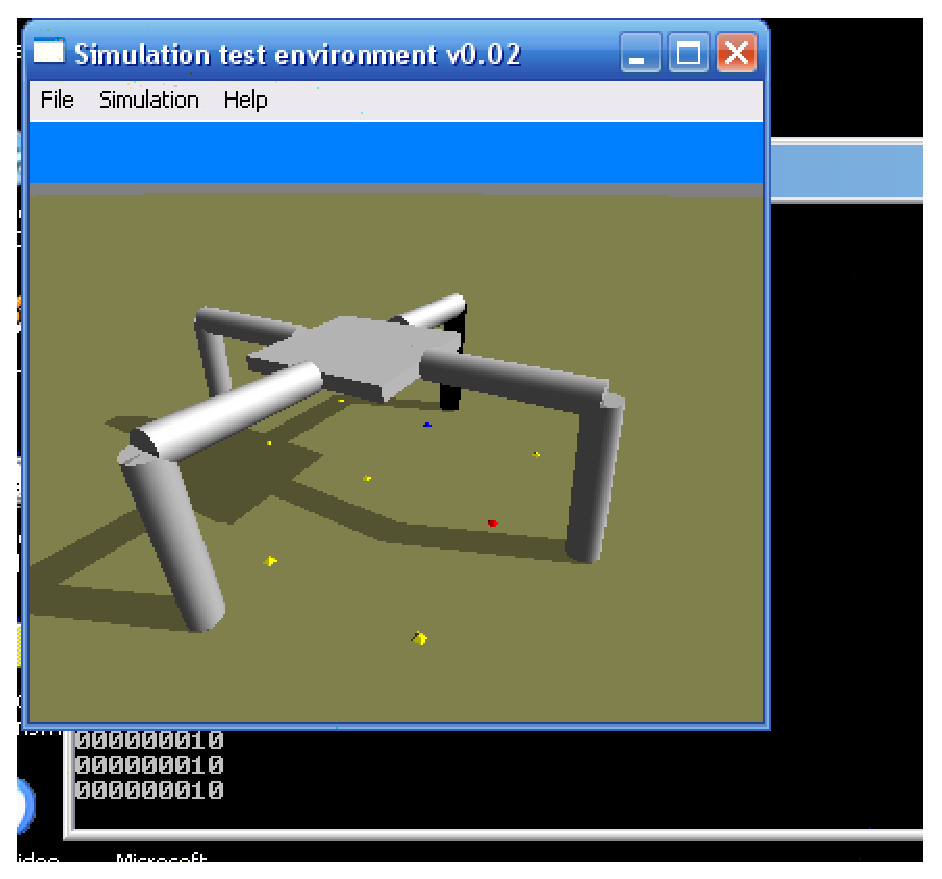
\includegraphics[height=5cm]{Quad3}}
\caption{Visual display of the touch sensors firing.}
\label{Fig1}
\end{figure}

The following instructions will realize these four steps.

\begin{enumerate}

\item Back up Assignment\_7 on a flash drive or another computer so that you can always return to your completed seventh assignment.

\item Copy directory Assignment\_7, which contains your submitted document and the entire ODE folder. Rename the new directory Assignment\_8.

\item ODE allows the user to associate a pointer with each ODE body using \\ \texttt{dBodySetData(dBodyID,void *data)}. You will create such a data structure, and store the ID of each ODE body there. That is, the third ODE object will have an ID of 3. At the top of the program, create an array of integers \texttt{int IDs[9]}.

\item Just after the array is created, set the $i$th element of the array to $i$.

\item In \texttt{CreateBox(...)} and \texttt{CreateCylinder(...)}, after the ODE body has been created, associate a pointer to the correct element in this array with the object: \\
    \texttt{dBodySetData(body[index],\&IDs[index]);}

\item Now, when \texttt{nearCallback} is called, you can determine which object is in contact with the ground plane. After these lines in \texttt{nearCallback} \\
    \texttt{int g1 = (o1 == ground );} \\
    \texttt{int g2 = (o2 == ground );} \\
    \texttt{if (!(g1 \^ g2)) return;}, \\
    one (but not both) of the objects is an ODE body, and the other is the ground plane.
    Within the code clause that is executed if a collision has actually occurred---that is, after \\
    \texttt{n = dCollide (o1,o2,N,\&contact[0].geom,sizeof(dContact));}\\
    \texttt{if (n > 0) \{}\\
    Add some code to check which object is the ground plane, and then get the user data from the \textit{other} object. For example if o1 is the ground plane, then o2 is an ODE body. You can get the ID of o2 using \\
    \texttt{int *IDPointer;}\\
    \texttt{...}\\
    \texttt{IDPointer = (int*)dBodyGetData(dGeomGetBody(o2));}\\
    If o2 is the ground plane, then you need to get the ID of o1.

\item Once you have this ID, print it to the output terminal:\\
    \texttt{printf("\%d $\backslash$n",*IDPointer);}. You should get something like the following when the simulation is running unpaused:\\
    \texttt{5}\\
    \texttt{7}\\
    \texttt{...}\\
    \texttt{6}\\
    If the robot is moving randomly (Fig. \ref{Fig1}), only the four lower legs (with IDs 5,6,7 and 8) will come into contact with the ground plane.

\item Now, at the top of the program, create a new integer array that will store the values of the four touch sensors:\\
    \texttt{int touches[9];} \\
    \texttt{touches[i]} will be set to 1 when the touch sensor in the $i$th body part is firing, and zero otherwise. Only \texttt{touches[5]} through \texttt{touches[8]} will be used, because the first five body parts do not have touch sensors.

\newpage

\item Calls to \texttt{simLoop} and \texttt{nearCallback} alternate: After one pass through \texttt{simLoop} completes, all of the \texttt{nearCallback} calls are made. Once they are complete, a new pass through \texttt{simLoop} is made, and so on. So, we need to set all of the touch sensors to zero at the end of \texttt{simLoop}, and then set all of the touch sensors that are firing to one during the \texttt{nearCallback} calls. Thus, when \texttt{simLoop} begins, all elements in \texttt{touches} are set correctly. First, back in \texttt{nearCallback}, after the print statement you can set the corresponding touch sensor as follows:\\
    \texttt{printf("\%d $\backslash$n",*IDPointer);}\\
    \texttt{touches[*IDPointer] = 1;}

\item Now, at the very end of \texttt{simLoop}, add a \texttt{for} loop that sets each element of \texttt{touches} to zero.

\item Somewhere within the \\
    \texttt{if ( !pause ) \{}\\
    clause of \texttt{simLoop} create a \texttt{for} loop that prints out the values of \texttt{touches}. When the simulation is run it should produce something like: \\
    \texttt{00001101}\\
    \texttt{00000101}\\
    \texttt{...}\\
    \texttt{00001000}\\
    (You can see this in Fig. \ref{Fig1}).

\item Now, within \texttt{DrawCylinder(i)}, you can include an \texttt{if} clause that will draw the $i$th cylinder black\\
    \texttt{dsSetColor (0,0,0);}\\
    if the $i$th element of \texttt{touches} is one, and draw it white\\
    \texttt{dsSetColor (1,1,1);}\\
    otherwise. When you compile and run the simulation, you should see that whenever a lower leg comes in contact with the ground it turns black, and turns white when it is lifted above the ground. Capture three images showing different legs doing this as in Fig. \ref{Fig1}, copy them into your document and submit to the T.A.

\end{enumerate}

\end{document} 
